
+%
% teil1.tex -- Beispiel-File für das Paper
%
% (c) 2020 Prof Dr Andreas Müller, Hochschule Rapperswil
%
% !TEX root = ../../buch.tex
% !TEX encoding = UTF-8
%
\section{Schallintensität
\label{helmholtz:section:teil1}}
\kopfrechts{Problemstellung}


\subsection{in der Praxis -> überabeiten besseres Beispiel}

Warum sollte die Schallintensität gemessen werden? Ein Anwendungsbeispiel besteht darin, die Gegenmassnahmen zu ergreifen, wenn an einem Arbeitsplatz die Lärmbelastung in einer Fabrikhalle den Grenzwert überschreitet. Hierzu ist es erforderlich, dass die Schallleistung einer jeden Maschine zu bestimmen, um die lauteste zu identifizieren.  \newline

Hierzu eignen sich Schallintensitätmessung, da sich diese in jeder Umgebung messen lässt, unabhängig von der akustischen Eigenschaft der Raumes. Stationäre Hintergrundgeräusche haben keinen Einfluss auf die Intensitätsmessung und somit auch nicht auf die Schallleistungswerte bei idealen Bedingungen (z. B. unkorreliertes, gleichfrequentes Rauschen, ausreichende Messdauer, etc.). Da die Schallintensität ist eine vektorielle Grösse ist, die sowohl Betrag als auch Richtung besitzt, ist sie hilfreich in der Schallquellenlokalisierung.

\begin{itemize}
\item Noise Source Identification (NSI) in der Automobilindustrie: https://www.sciencedirect.com/science/article/pii/S0003682X11003045?via%3Dihub
\item Lärmbekämpfung in Windkraftanlagen
\item 
\end{itemize}



\subsection{Ebene Welle $\mathbf{Q} = 0$
\label{helmholtz:subsection:ebeneWelle}}

Ebene Welle bedeutet, dass ...
\begin{enumerate}
\item bei einer planaren Welle ist $P (\mathbf{r}) = A = konst.\quad bzw. \quad \nabla P = 0$.
\item Aus der Gleichung \eqref{helmholtz:equationReaktiveIntensitaet} folgt $\mathbf{Q} = \mathbf{0}$.
\item sowie aus der Gleichung \eqref{helmholtz:equationAktiveIntensitaet} folgt $\mathbf{I} \neq \mathbf{0}$ da $ \nabla \phi$ parallel zur Ausbreitungsrichtung ist. In diesem Fall ergibt sich die aktive Intensität zu: $\mathbf{I} = \frac{|\mathbf{A}|^2}{2 \rho_0 c_0}$
\item Schalldruck $P$ und Schall-Schnelle $v$ sind in Phase ($\phi = 0^{\circ}$).
\end{enumerate}


\begin{equation}
	\mathbf{I}_c ~(\mathbf{r}) = \underbrace{\mathbf{I}~(\mathbf{r})}_{\textit{aktive Intensität}} + \underbrace{ \cancel{j\,\mathbf{Q}~(\mathbf{r})}}_{\textit{reaktive~Intensität}~=~0}.
	\label{helmholtz:equationIntensitaetComplexplanar}
\end{equation}	


\subsection{stehende Welle $\mathbf{I} = 0,\mathbf{Q} \neq 0$
\label{helmholtz:subsection:stehendeWelle}}

Bei einer stehenden Welle überlagern (Superposition) sich zwei gleiche planare Wellen mit gleicher Amplitude in entgegengesetzter Richtung und hat folgende Charakteristik:

\begin{enumerate}
\item an jedem Punkt ist entweder  $P = maximal$ und $v = 0$ bei einem Bauch (Darstellung) oder $P = 0$  und $ v = maximal$ bei einem Knoten (Darstellung).
\item fehlt noch was ??
\item Schalldruck $P$ und Schall-Geschwindigkeit $v$ sind 90\textdegree phasenverschoben ($\phi = 90^{\circ}$).
\end{enumerate}



\begin{equation}
	\mathbf{I}_c ~(\mathbf{r}) = \underbrace{\cancel{\mathbf{I}~(\mathbf{r})}}_{\textit{aktive Intensität}~=~0} + \underbrace{j\,\mathbf{Q}~(\mathbf{r})}_{\textit{reaktive~Intensität}}
	\label{helmholtz:equationIntensitaetComplexStehend}
\end{equation}	

\begin{figure}[h!]
	\centering
	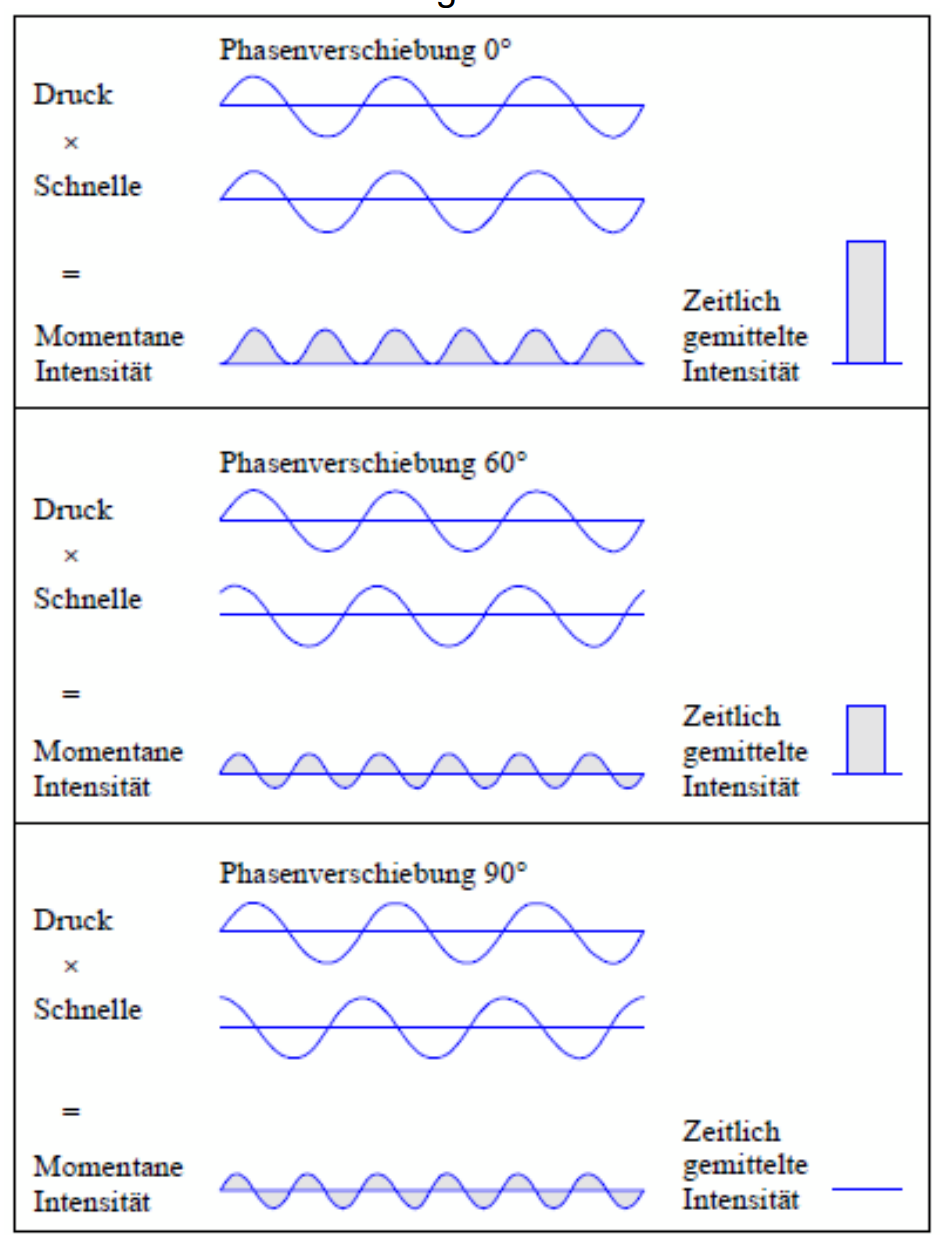
\includegraphics[scale=0.4]{papers/helmholtz/images/Schallintensitaet.png}
	\caption{Schallintensität Beispiel}
	\label{fig:LaplaceAlg}
\end{figure}